\documentclass[pdftex,12pt,a4paper]{article}
\usepackage{amsthm}
\usepackage{amssymb}
\usepackage{enumerate}
\usepackage{amsmath}
\usepackage{verbatim}
\usepackage{graphicx}
\usepackage{hyperref}
\usepackage{fancyhdr}

\newcommand{\HRule}{\rule{\linewidth}{0.5mm}}


\pagestyle{fancy}

\fancyhead[RO,RE]{Peter Zhang and Carl Jackson}
\fancyhead[LO, RE]{CS 171: Project 2}

\begin{document}
\begin{titlepage}
\begin{center}

% Upper part of the page. The '~' is needed because \\
% only works if a paragraph has started.

\includegraphics[width=0.15\textwidth]{twitterlogo.jpg}~\\[1cm]


\textsc{\Large CS 171: Project 2}\\[0.5cm]

% Title
\HRule \\[0.4cm]
{ \LARGE \bfseries Pheme: \\ Birds of a Feather Tweet Together} \\[0.4cm]

\HRule \\[1.5cm]

% Author and supervisor
\begin{minipage}{0.6\textwidth}
\begin{flushleft} \large
\emph{Authors:}\\
Carl Jackson and Peter Zhang
\end{flushleft}
\end{minipage}
\begin{minipage}{0.4\textwidth}
\begin{flushright} \large
\end{flushright}
\end{minipage}

\vfill

% Bottom of the page
{\large \today}

\end{center}
\end{titlepage}
\tableofcontents
\pagebreak

\section{Introduction}
\subsection{Motivation}
Most current visualizations of social data require viewers to already have a subject matter in mind; they allow viewers to search for and investigate specific keywords, hashtags, or locales. However, we think that social data is interesting primarily because it allows us to discover new topics for investigation - topics that are being generated in real time by the humans who are producing the social data. Accordingly, we want to build a visualization that guides a curious but unfocused viewer in identifying undiscovered topics/events that are currently occurring in the real world.
\subsection{Goals}
In this project, our goal is to investigate high-throughput social data streams, and answer two primary research questions:
\begin{enumerate}
\item Can we identify "events" from real-time social data?
\item If we can, what can we learn about such "events" from various social data sources?
\end{enumerate}
To achieve these goals, we have built a visualization that tries to identify current events that are occurring within a user-specified geography (location + radius), using real time social data. Concretely, we pull a live stream of Twitter data being generated in the specified geography, and try to identify clusters of tweets; currently, we cluster primarily by geographical proximity, but hope to cluster using other techniques in project 3. Currently, we aren't doing significant processing on the events that we identify, but we hope to expand on that in project 3.

\section{Description of Data}
\subsection{Source}
The ultimate source of the data for our visualizations is Twitter, an online social network and microblogging service that allows users to instantaneously send and receive short messages, called tweets, on various electronic devices. Twitter is one of the most popular, if not the most popular, sites that produces real-time social data; as of 2012, it produced more than 340 million tweets per day \footnote{http://techcrunch.com/2012/07/30/analyst-twitter-passed-500m-users-in-june-2012-140m-of-them-in-us-jakarta-biggest-tweeting-city/}. Given our interest high-throughput social data streams, Twitter was a natural data source to focus on.

Using Twitter's API, we pulled tweets, which contained several relevant pieces of information:
\begin{enumerate}
\item Geographical location: Twitter users can choose to specify a geographical location to associate with their tweet. This is particularly interesting for users who tweet on their mobile phones, and choose to expose their phone's GPS data to the service.
\item Twitter Screenname: Tweets are associated with the screen name of the user publishing the tweets.
\item Tweet contents: The actual text content of the tweet. This is also available to viewers of our visualization.
\item Hashtags: Twitter users can specify hashtags, or metadata, to associate with their tweet. 
\item Tweet timestamp: The time at which the tweet was published.
\end{enumerate}

\subsection{Scraping Method}

Typically, Twitter's API allows you to view historical tweets, at most a few
hundred at a time, using its REST API. Since we wanted to see tweets as they
happened, we instead chose to rely on Twitter's streaming API, which is a
mechanism by which you can express interest in a particular Twitter search
query, and receive push updates from Twitter as new Tweets are written that
match the query. This live stream is sometimes referred to as the ``Twitter
Firehose,'' although Twitter only makes a subsampling of the full Firehose
available for third party developers.

Twitter's streaming API allows you to search for tweets by geographical
location, so we established a connection to Twitter that requested the Tweets
that would be visible on the user's screen. Each user needed to have their
tweets scraped from a different live API feed, since different users can be
visualizing different portions of the map at once.

One particular challenge involved with Twitter's streaming feed was that of
authentication. Twitter protects their streaming API using OAuth, which is a
mechanism for authenticating individual Twitter users with third party
applications. In order to get access to a live stream of tweets, we must prove
to Twitter that we are doing it on behalf of a valid Twitter user, and obtaining
these credentials is a particularly finicky multi-step process. Only after
forcing users to authenticate can we proceed with our visualization.

\section{Related Work}
To the extent that we've used what we've learned so far in CS 171, all the readings and lecture materials are related work; when justifying our visualization choices or visualization evolution, we will refer to this material. We consulted documentation related to the Twitter API and the Google Maps API very often while working on this project. Finally, we were inspired to investigate and study tweets and their geographical data by a past CS 171 project: Tweetography. \\ \\
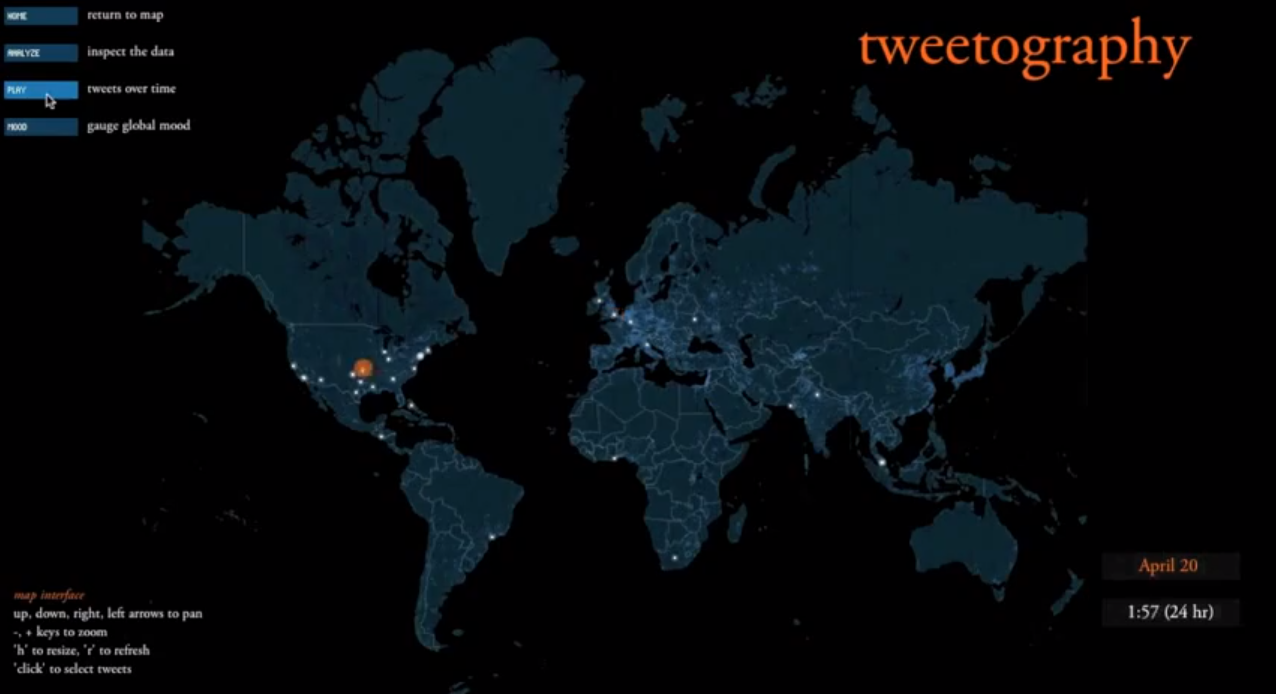
\includegraphics[width=5.5in]{tweetography.png} \\ \\
We found the concept of tweets appearing over time on a map very attractive, and based our visualization on this concept, even though the purpose and design of our visualization is very different than Tweetography.

\section{Design Evolution}
In our initial proposal, we envisioned a visualization where tweets, and clusters of tweets that have been identified as a cluster, are displayed on a map as they are generated; our initial sketch of how this might look is included below: \\ \\
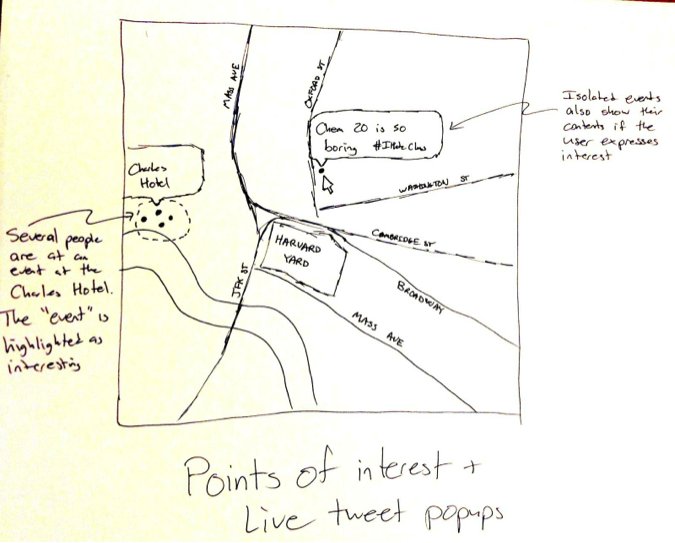
\includegraphics[width=5in]{proposal1.png} \\ \\
In addition, we imagined a sidebar that would display tweet and cluster information as they came in, similar to the image below: \\ \\
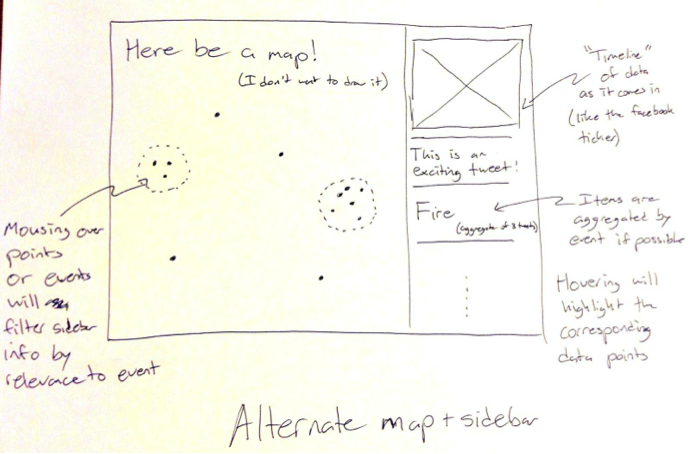
\includegraphics[width=5in]{proposal2.png} \\ \\
Throught the evolution of our visualization, these fundamental design choices have not changed. However, we did have to address specific design issues during this project.

\subsection{Maps}
First, we had to decide on the background of our visualization, the map. As covered in class and homework, there are several ways to draw maps using D3, including an SVG map from wikipedia or the datamaps add-on. We really liked D3, especially the way it binds data directly to elements of the DOM. However, we ultimately decided that D3 was not particularly suitable for our visualization, because we needed a very finely detailed map for our visualization. Since we desired to identify events and their geographical location, it was important for users to be able to see the exact street address of the tweets and events we were visualizating, as well as the surrounding buildings and other geographical features. For example, one event we ultimately identified while testing our visualization was the opening game at Fenway Park: \\ \\
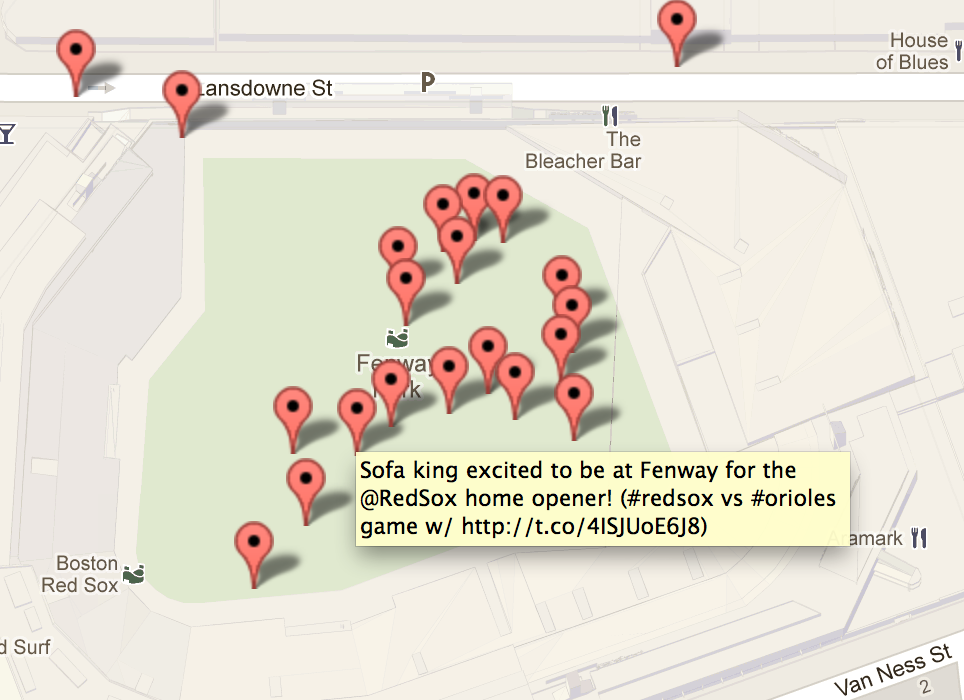
\includegraphics[width=5.5in]{fenway.png} \\
If the map we chose to visualize tweets on did not contain detailed city, street, and building information, it would have been much harder to understand exactly what and where this event was occurring.
Accordingly, we decided to build our visualization using the Google Maps API. In addition to a very detailed map, which would help viewers make a variety of useful visual queries relating to the events we identify, the Google Maps API contains several nice features, including zooming - which will allow users to drill down/filter as we explain later - and simple methods to draw basic objects on the map. 

\subsection{Clustering}
We faced two challenges when deciding how to construct and visualize our clusters.

\subsubsection{Clustering Algorithm}
Our first task was to decide how to actually identify clusters of tweets; we knew that clusters would be based on geographical distance, but needed to decide on a specific clustering algorithm. Most traditional clustering algorithms, like k-means clustering, hierarchical clustering, and autoclass clustering, do not fit our visualization goal. Not only do they depend on the assumption that all the points to be clustered are available immediately - which is not true in our case, because tweets arrive in realtime in our visualization - they also try to fit every point to a cluster - which is not what we desire, because we only want to cluster points that we believe are close enough to actually be an event. Accordingly, we designed the following simple algorithm for clustering:

First, we take the Cartesian distance between every two points in the system.
Any pairs which are below some threshold distance (in our testing, we found that
a distance of about 150 meters was appropriate), are considered part of the same
cluster. Once a cluster has more than some minimum number of points (say,
three), we emit it as a cluster, calculating its color, center, radius, and
other information.

By using a disjoint set data structure, we are able to maintain the information
about which points ought to be clustered with which other points in an efficient
manner. Furthermore, points can be considered as they arrive in an incremental
fashion, as the introduction of a single point creates only a few new edges. In
this fashion, we made our relatively simple clustering algorithm efficient
enough for use with hundreds if not thousands of data points.

\subsubsection{Visualizing Clusters}
Once we decided upon the algorithm by which we would identify clusters, we had to decide how to visualize them. 

Initially, we considered leaving tweets as the original google maps marker, and connecting tweets in a cluster with lines. On the one hand, this would allow viewers to see how the cluster grew with time, as lines would extend out from old tweets in the cluster to new tweets in the cluster. However, there were a significant drawbacks to this method. On a relatively zoomed out map, it would be difficult to actually identify clusters by eye on the map because all the tweet markers would look the same, and the lines connecting tweets would be extremely small; this visual query is particularly important to our viewers.

To address this problem, we decided to encode cluster membership using color; tweets would normally appear as blue dots on the map, and change colors once they were associated with a particular cluster, so that each cluster has a different color. We selected a color scheme using Color Brewer, as recommended in lecture;\footnote{http://colorbrewer2.org/} we set Color Brewer to $12$ data classes, the maximum, and specified that the nature of our data was qualitative. Every cluster would be randomly assigned a unique color from our color scheme as it was generated, and tweets in that cluster would be colored accordingly. At this stage, our visualization looked like the following: \\ \\
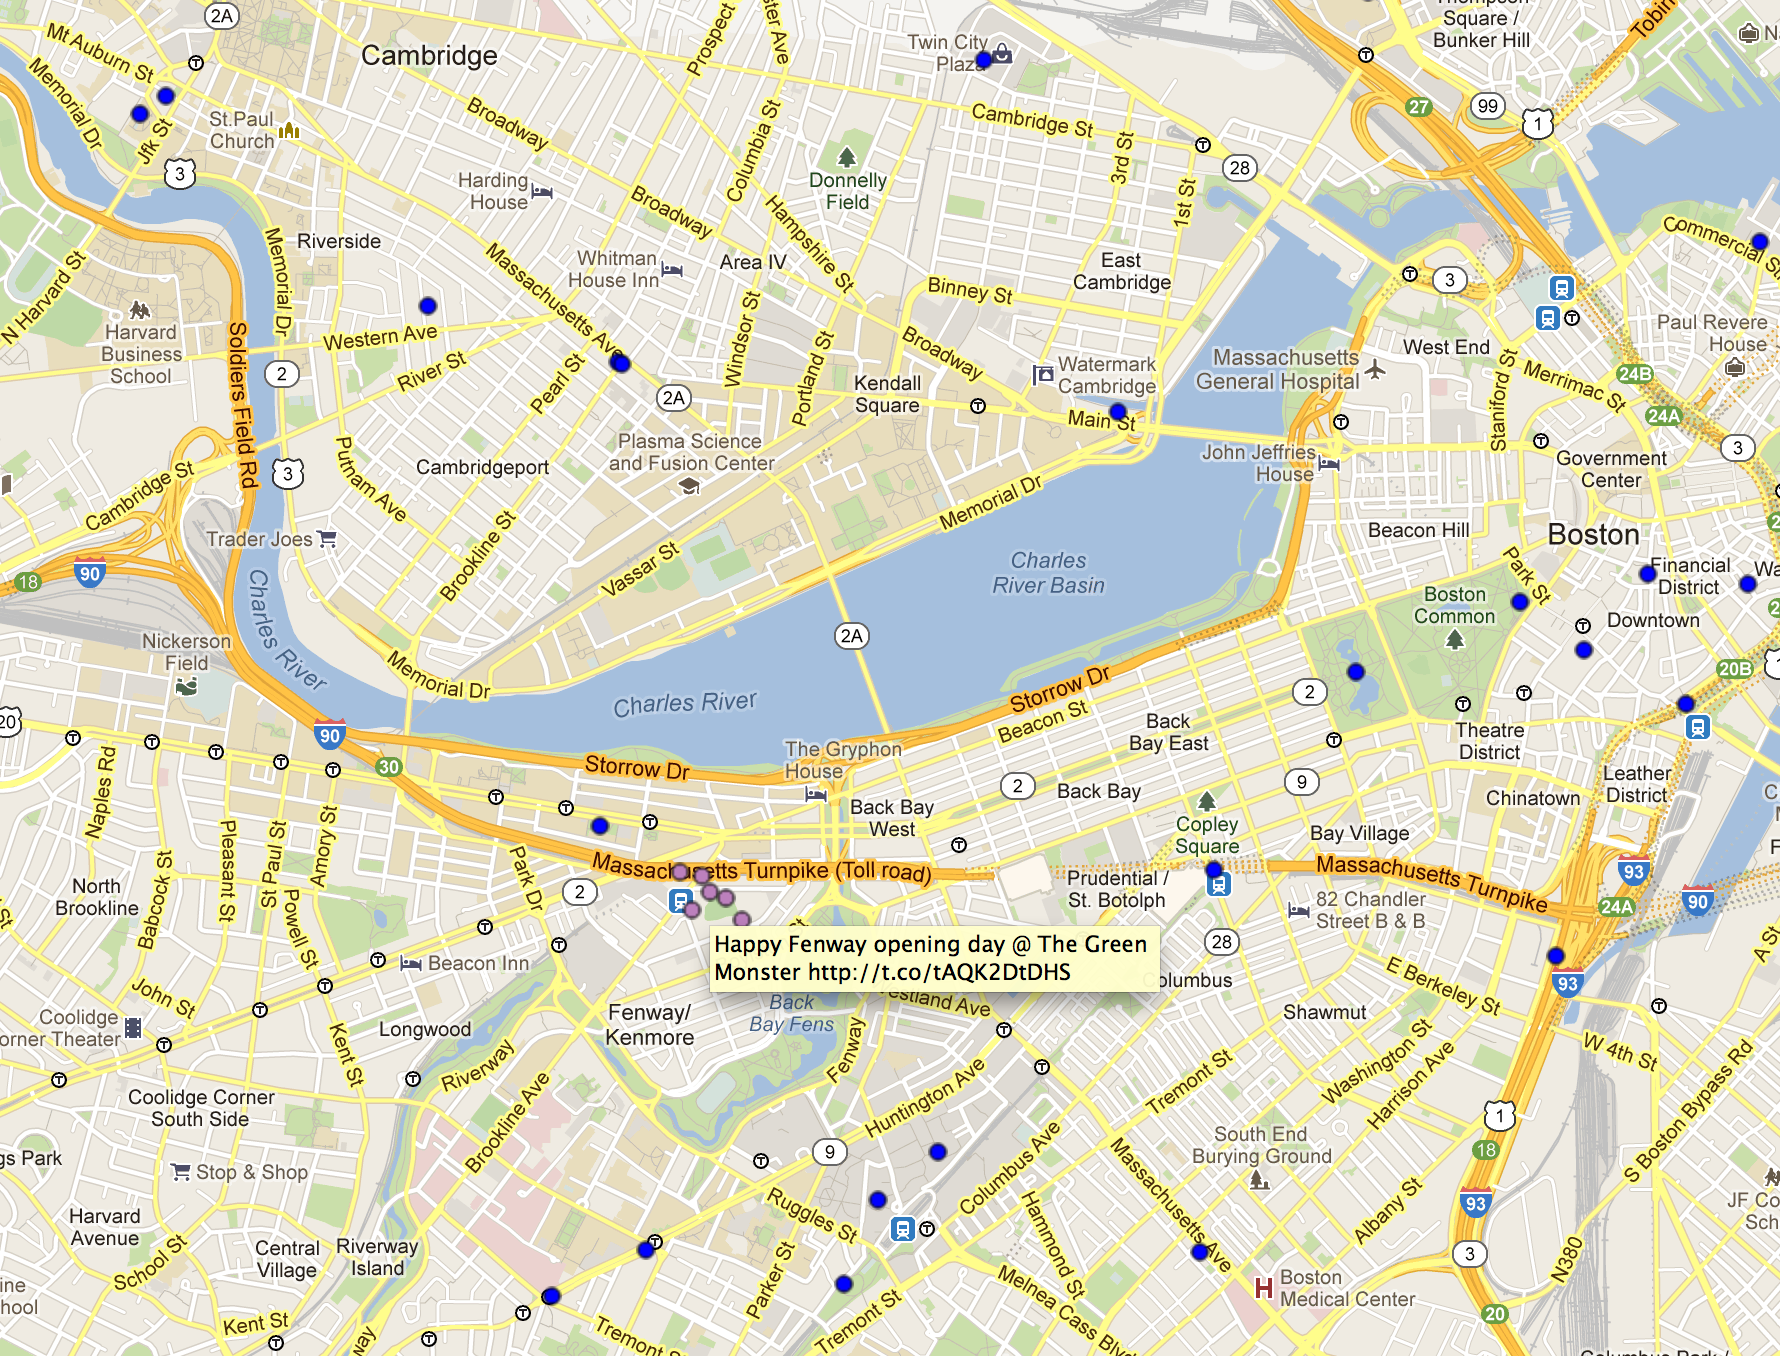
\includegraphics[width=5.5in]{fail1.png} \\ \\
At this zoom it's relatively easy to identify the cluster (in purple); we made sure that multiple tweets from exactly the same location would not show up on top of each other by providing some very small random noise in the location of the tweet. Unfortunately at lower zooms, all of the tweets in the cluster are on top of each other, so it is one purple dot in a sea of blue dots.
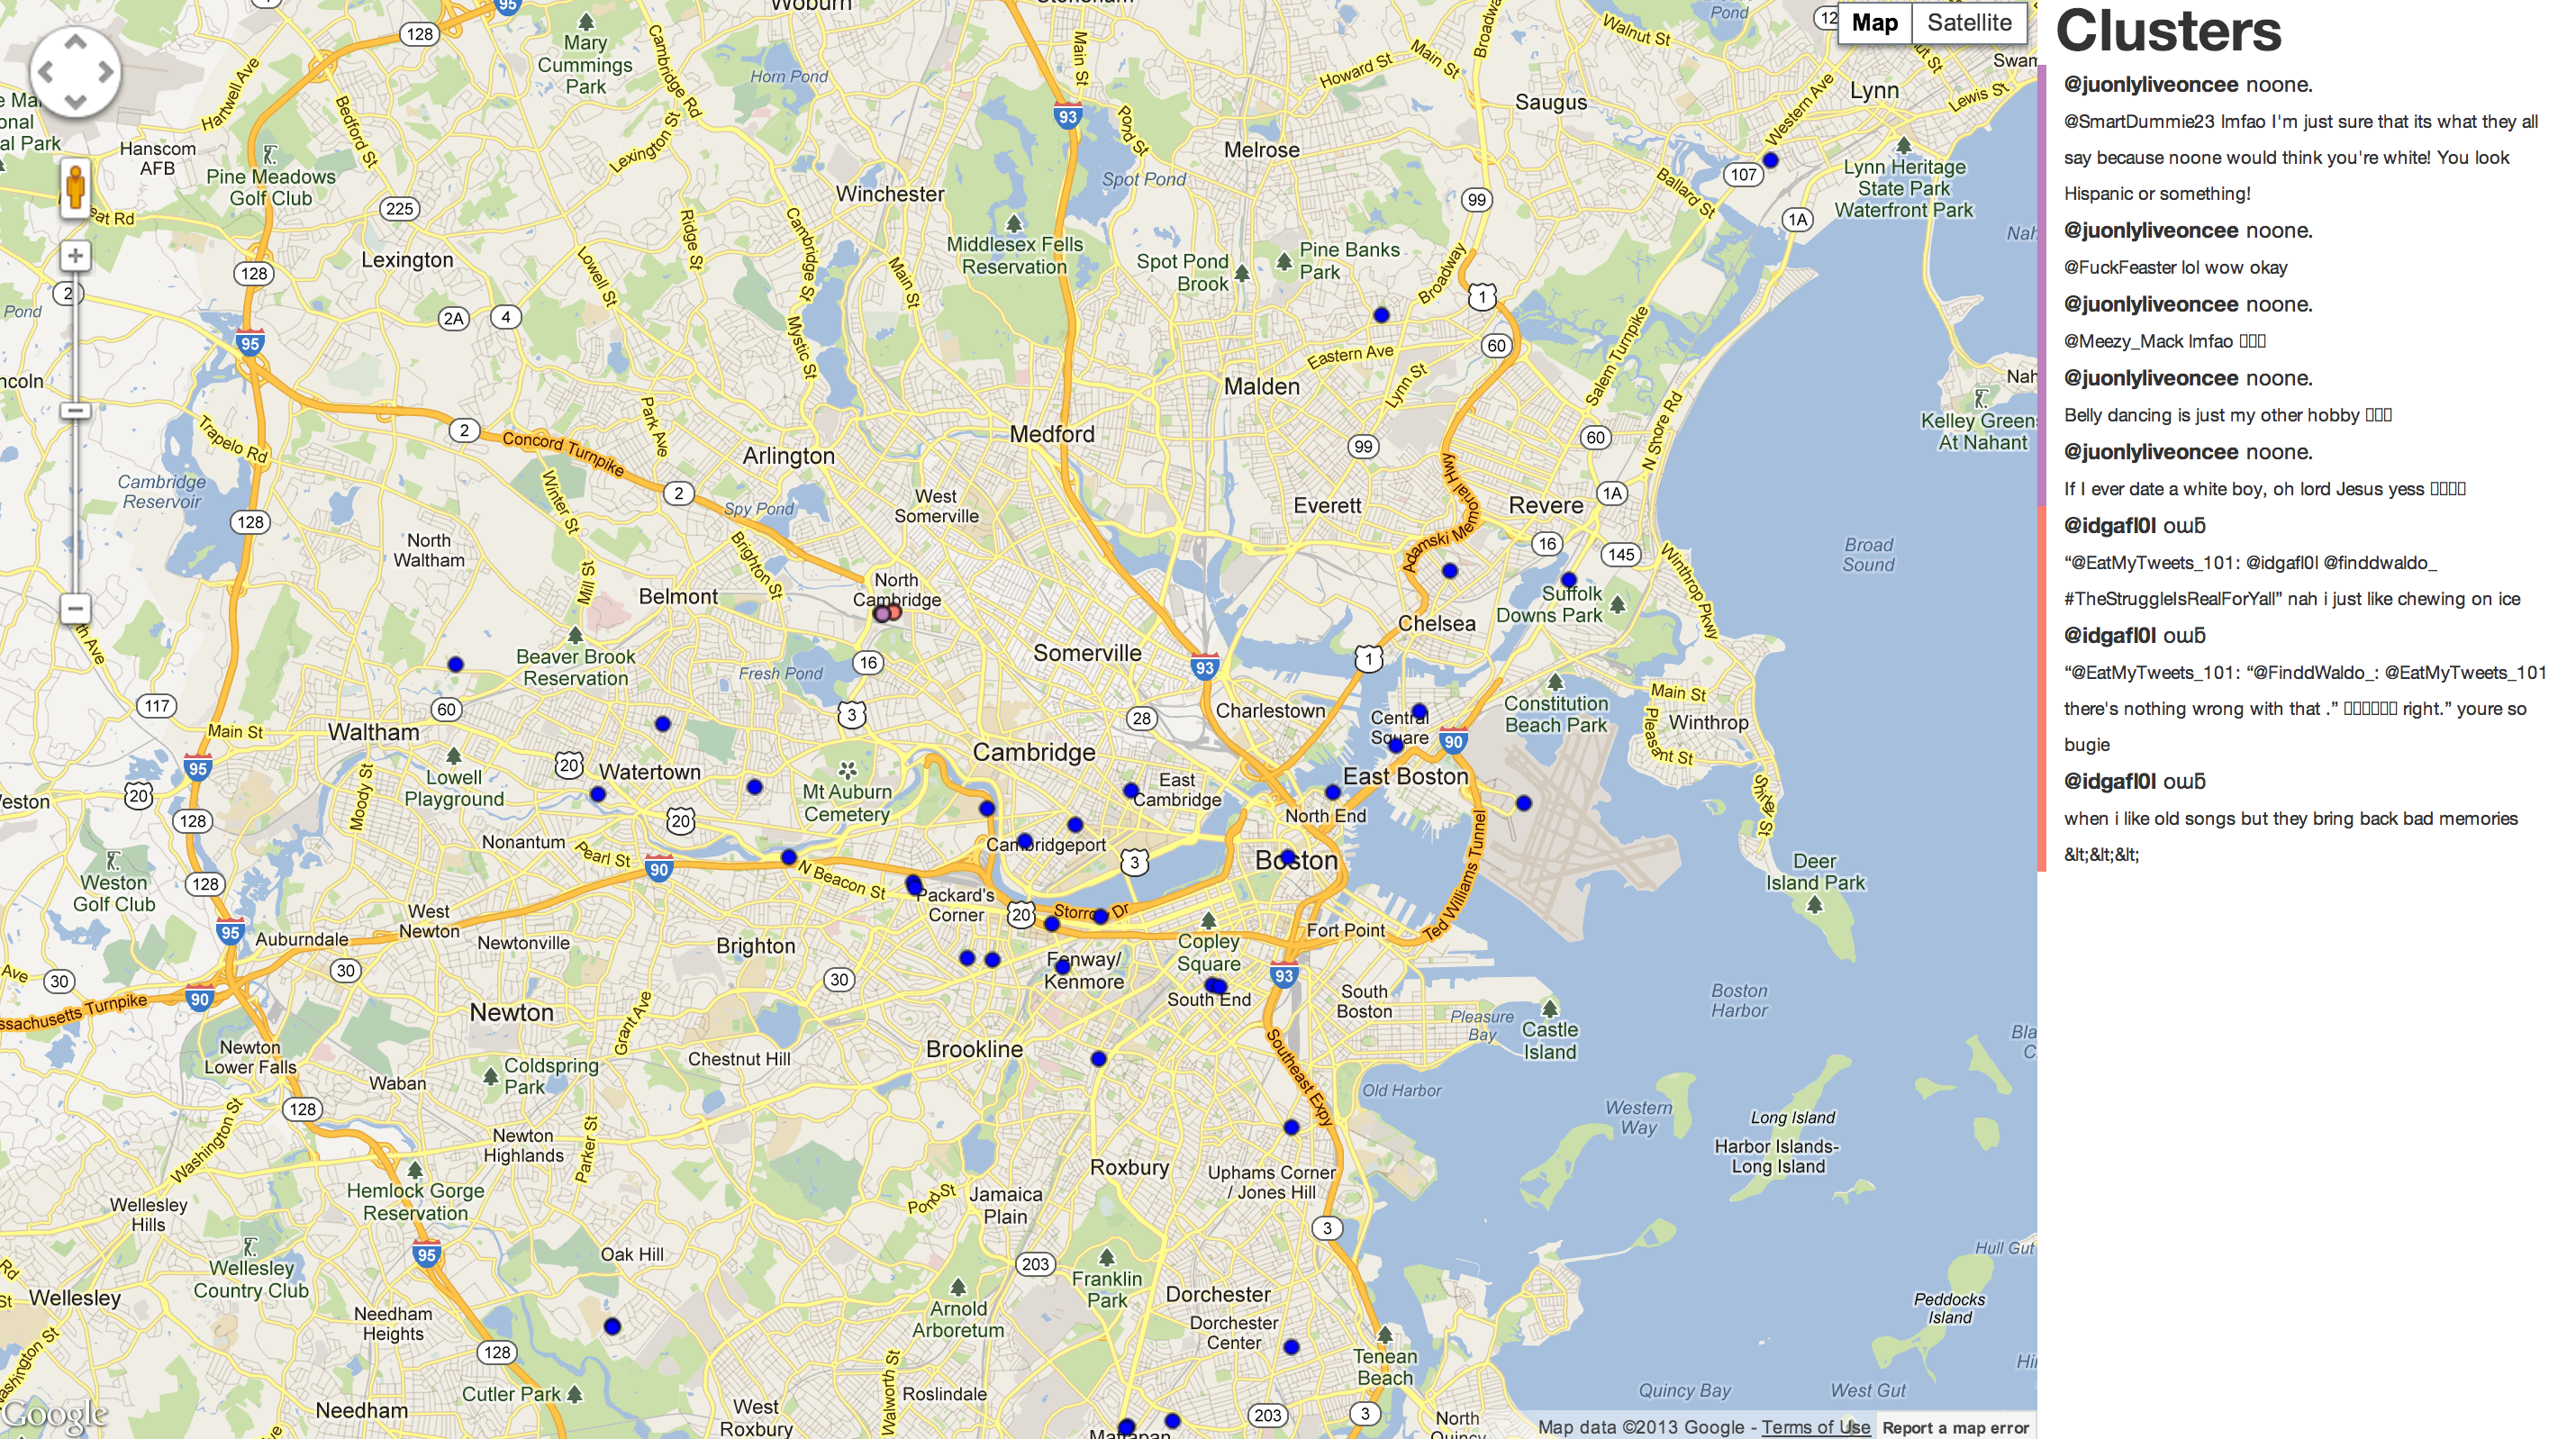
\includegraphics[width=5.5in]{fail2.png} \\ \\
Obviously, while better than the previous idea, viewers would still certainly have trouble identifying this cluster by eye at higher zooms. Furthermore, even at the higher zoom, users faced another two issues. First, they can't easily visually identify the center and size of the cluster. Second, viewers cannot distinguish between brushing or selecting an individual tweet, and brushing or selecting a cluster.

Accordingly, we iterated on our visualization once more. To help viewers actually visualize the cluster itself, rather than only the constituent tweets, we decided to compute the center of every cluster (the average of the longitude and latitude of every tweet in the cluster) and the radius of every cluster (the distance between the center of the cluster and the tweet in the cluster that is furtherest away from the center). Then, we drew a translucent circle in the current cluster's color with center and radius as calculated above, so that viewers of our visualization could actually see the clusters the visualization had identified. \\ \\
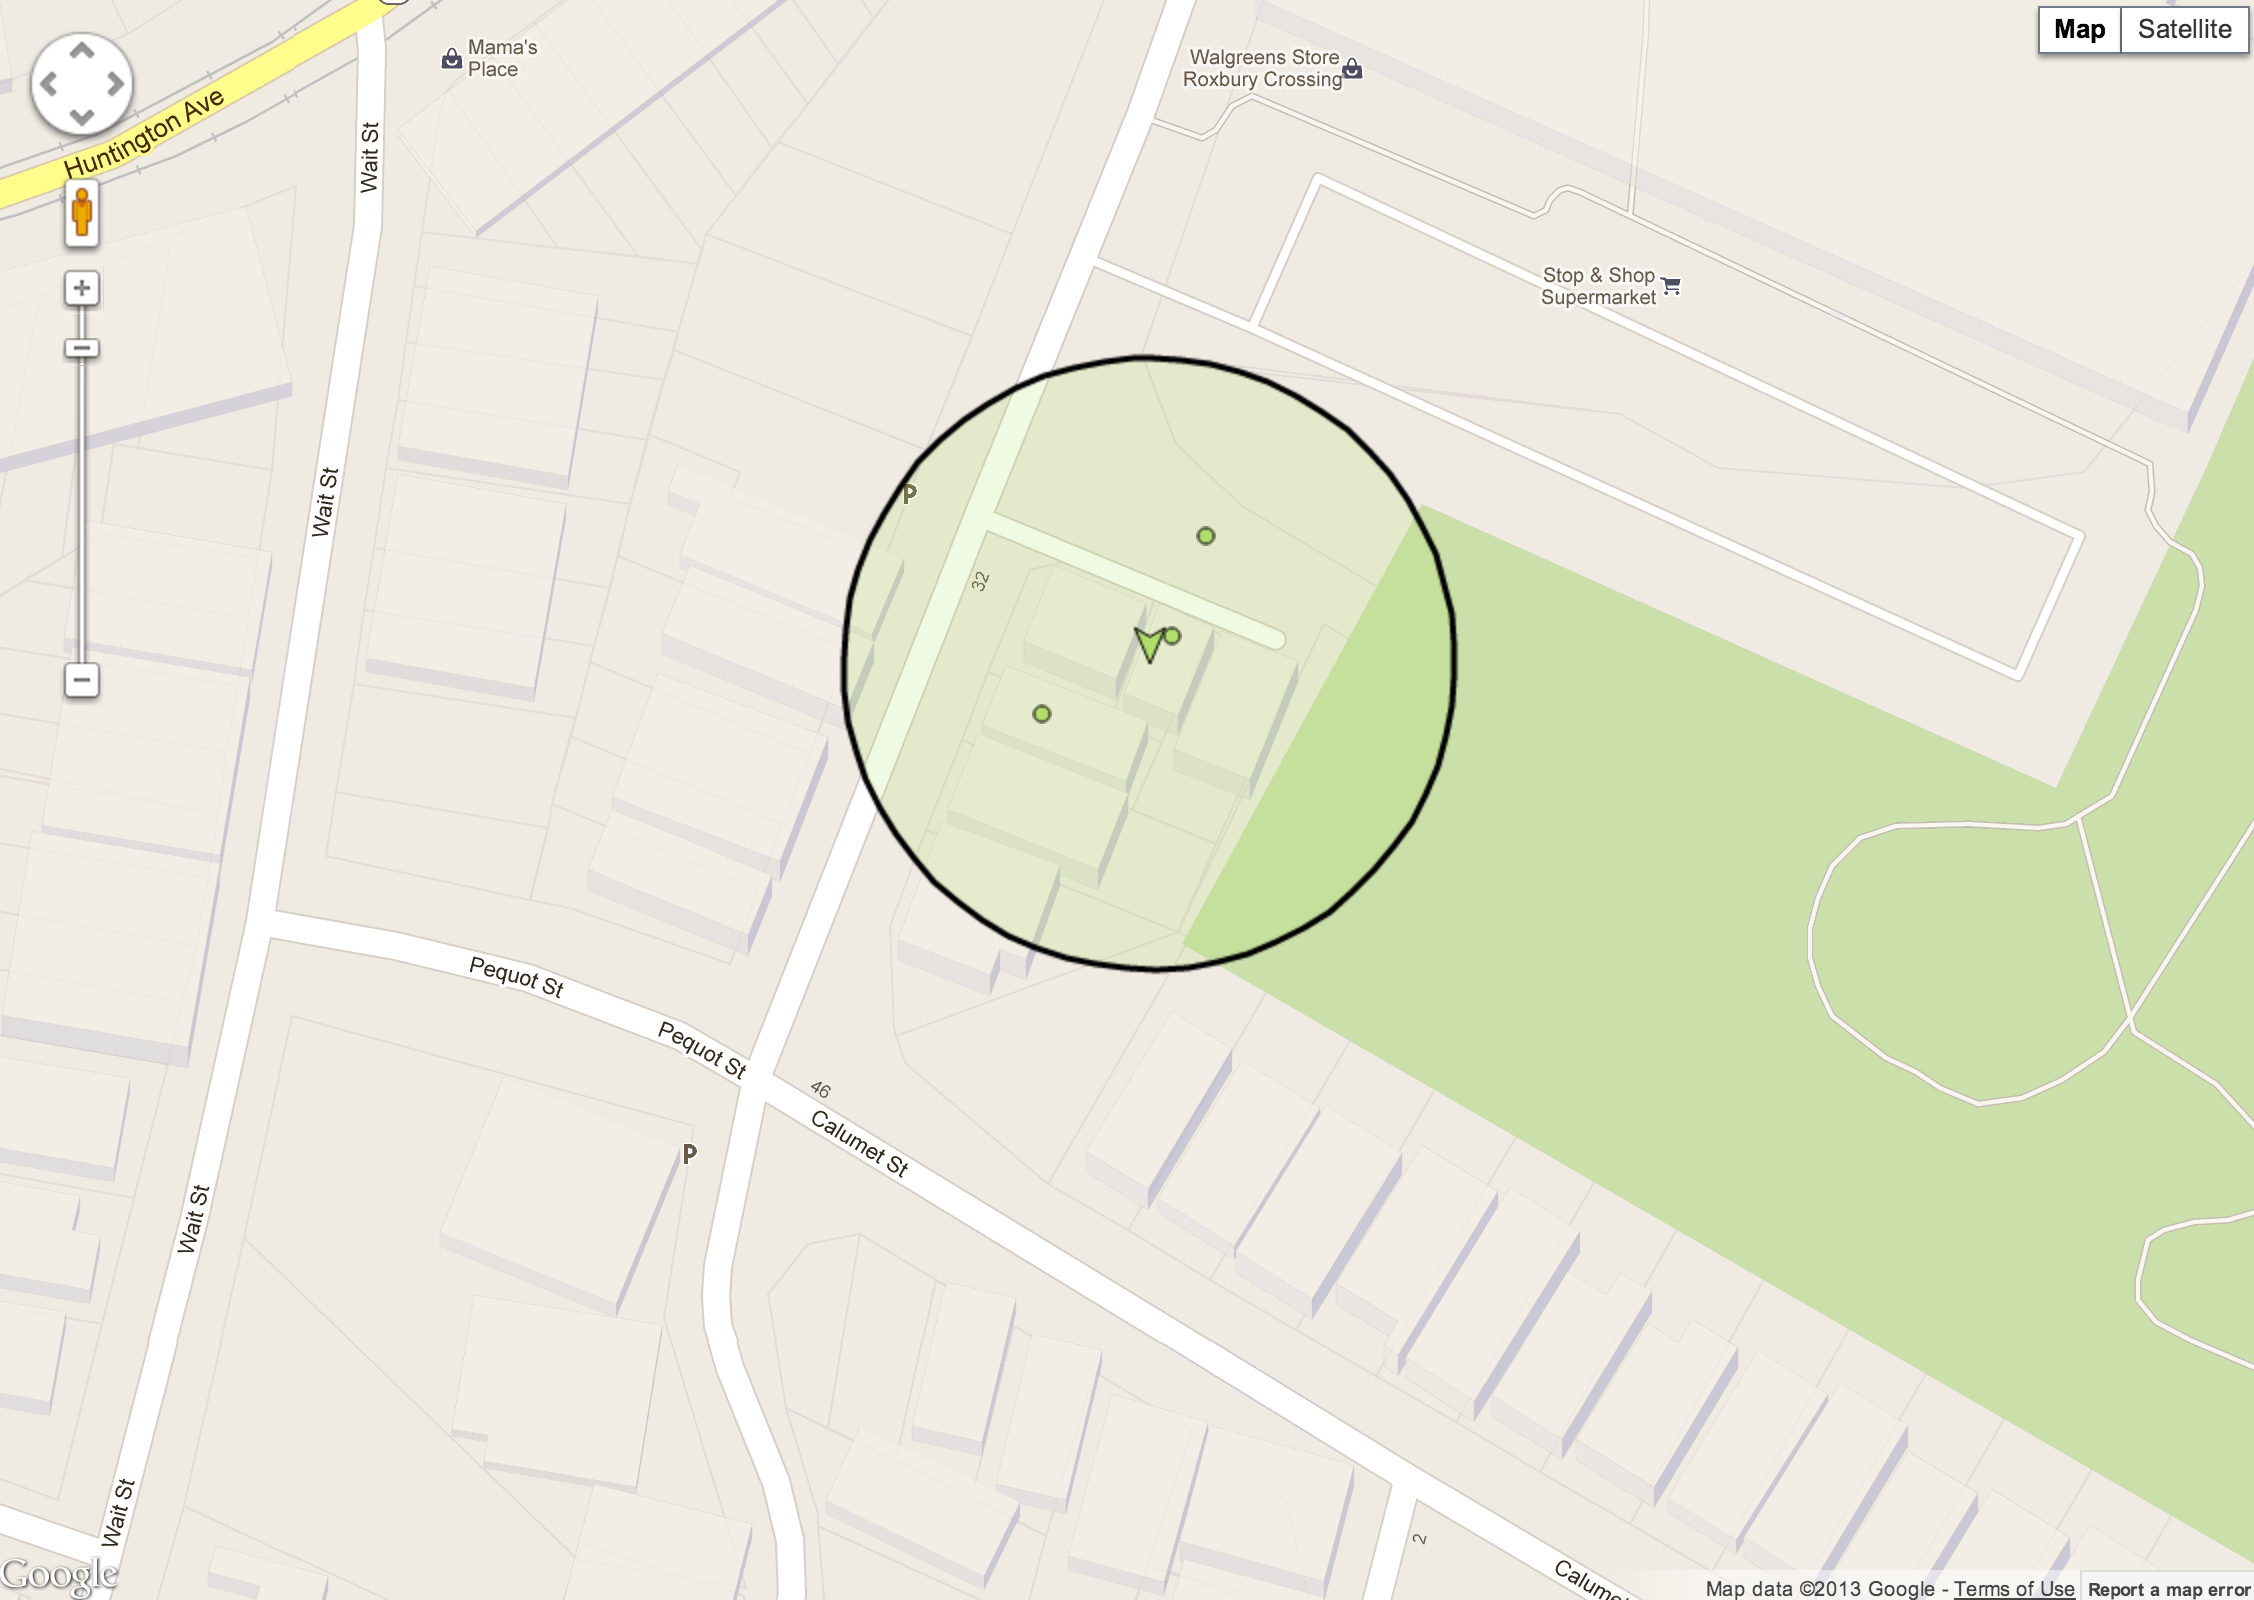
\includegraphics[width=5.5in]{success1.png} \\ \\
To help viewers distinguish between brushing or selecting an individual tweet, and brushing or selecting a cluster, we placed a marker of the appropriate color at the center of every cluster. In this way, viewers can hover over the cluster in the sidebar to enlarge the cluster marker on the map (shown below). \\ \\
Hovering over a cluster: \\
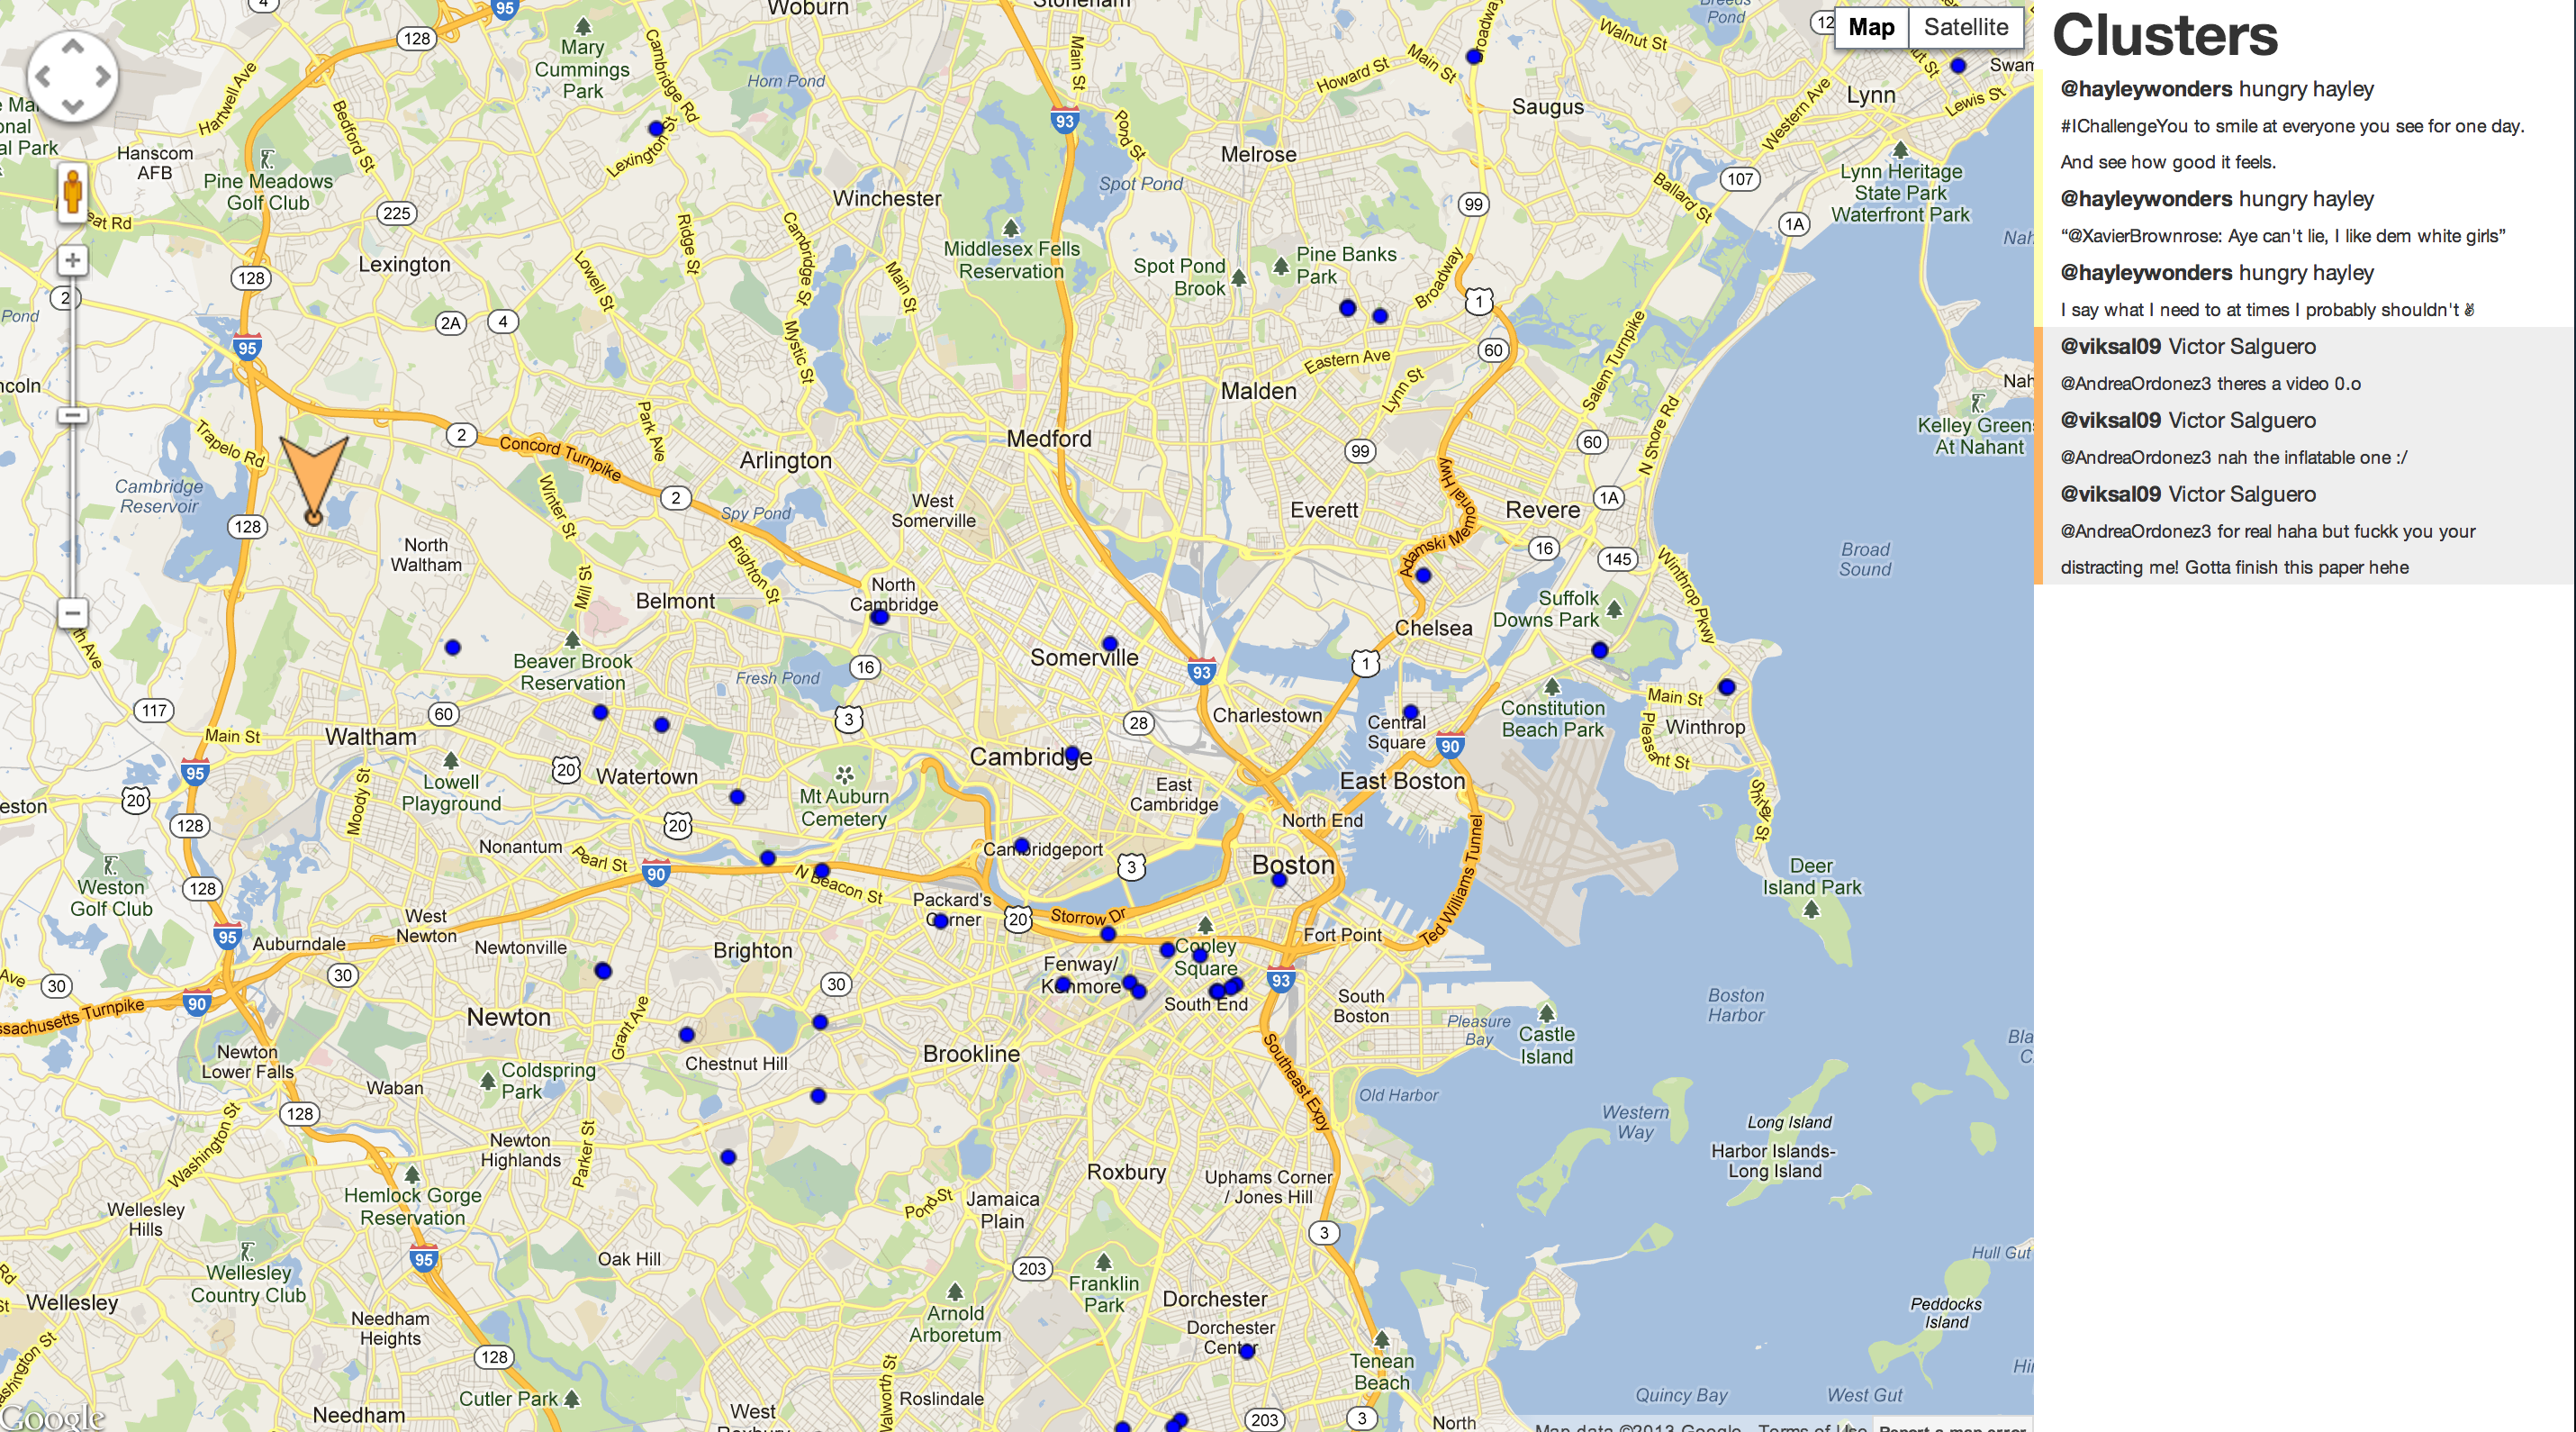
\includegraphics[width=5.5in]{hover1.png} \\ \\
Not hovering over a cluster: \\ 
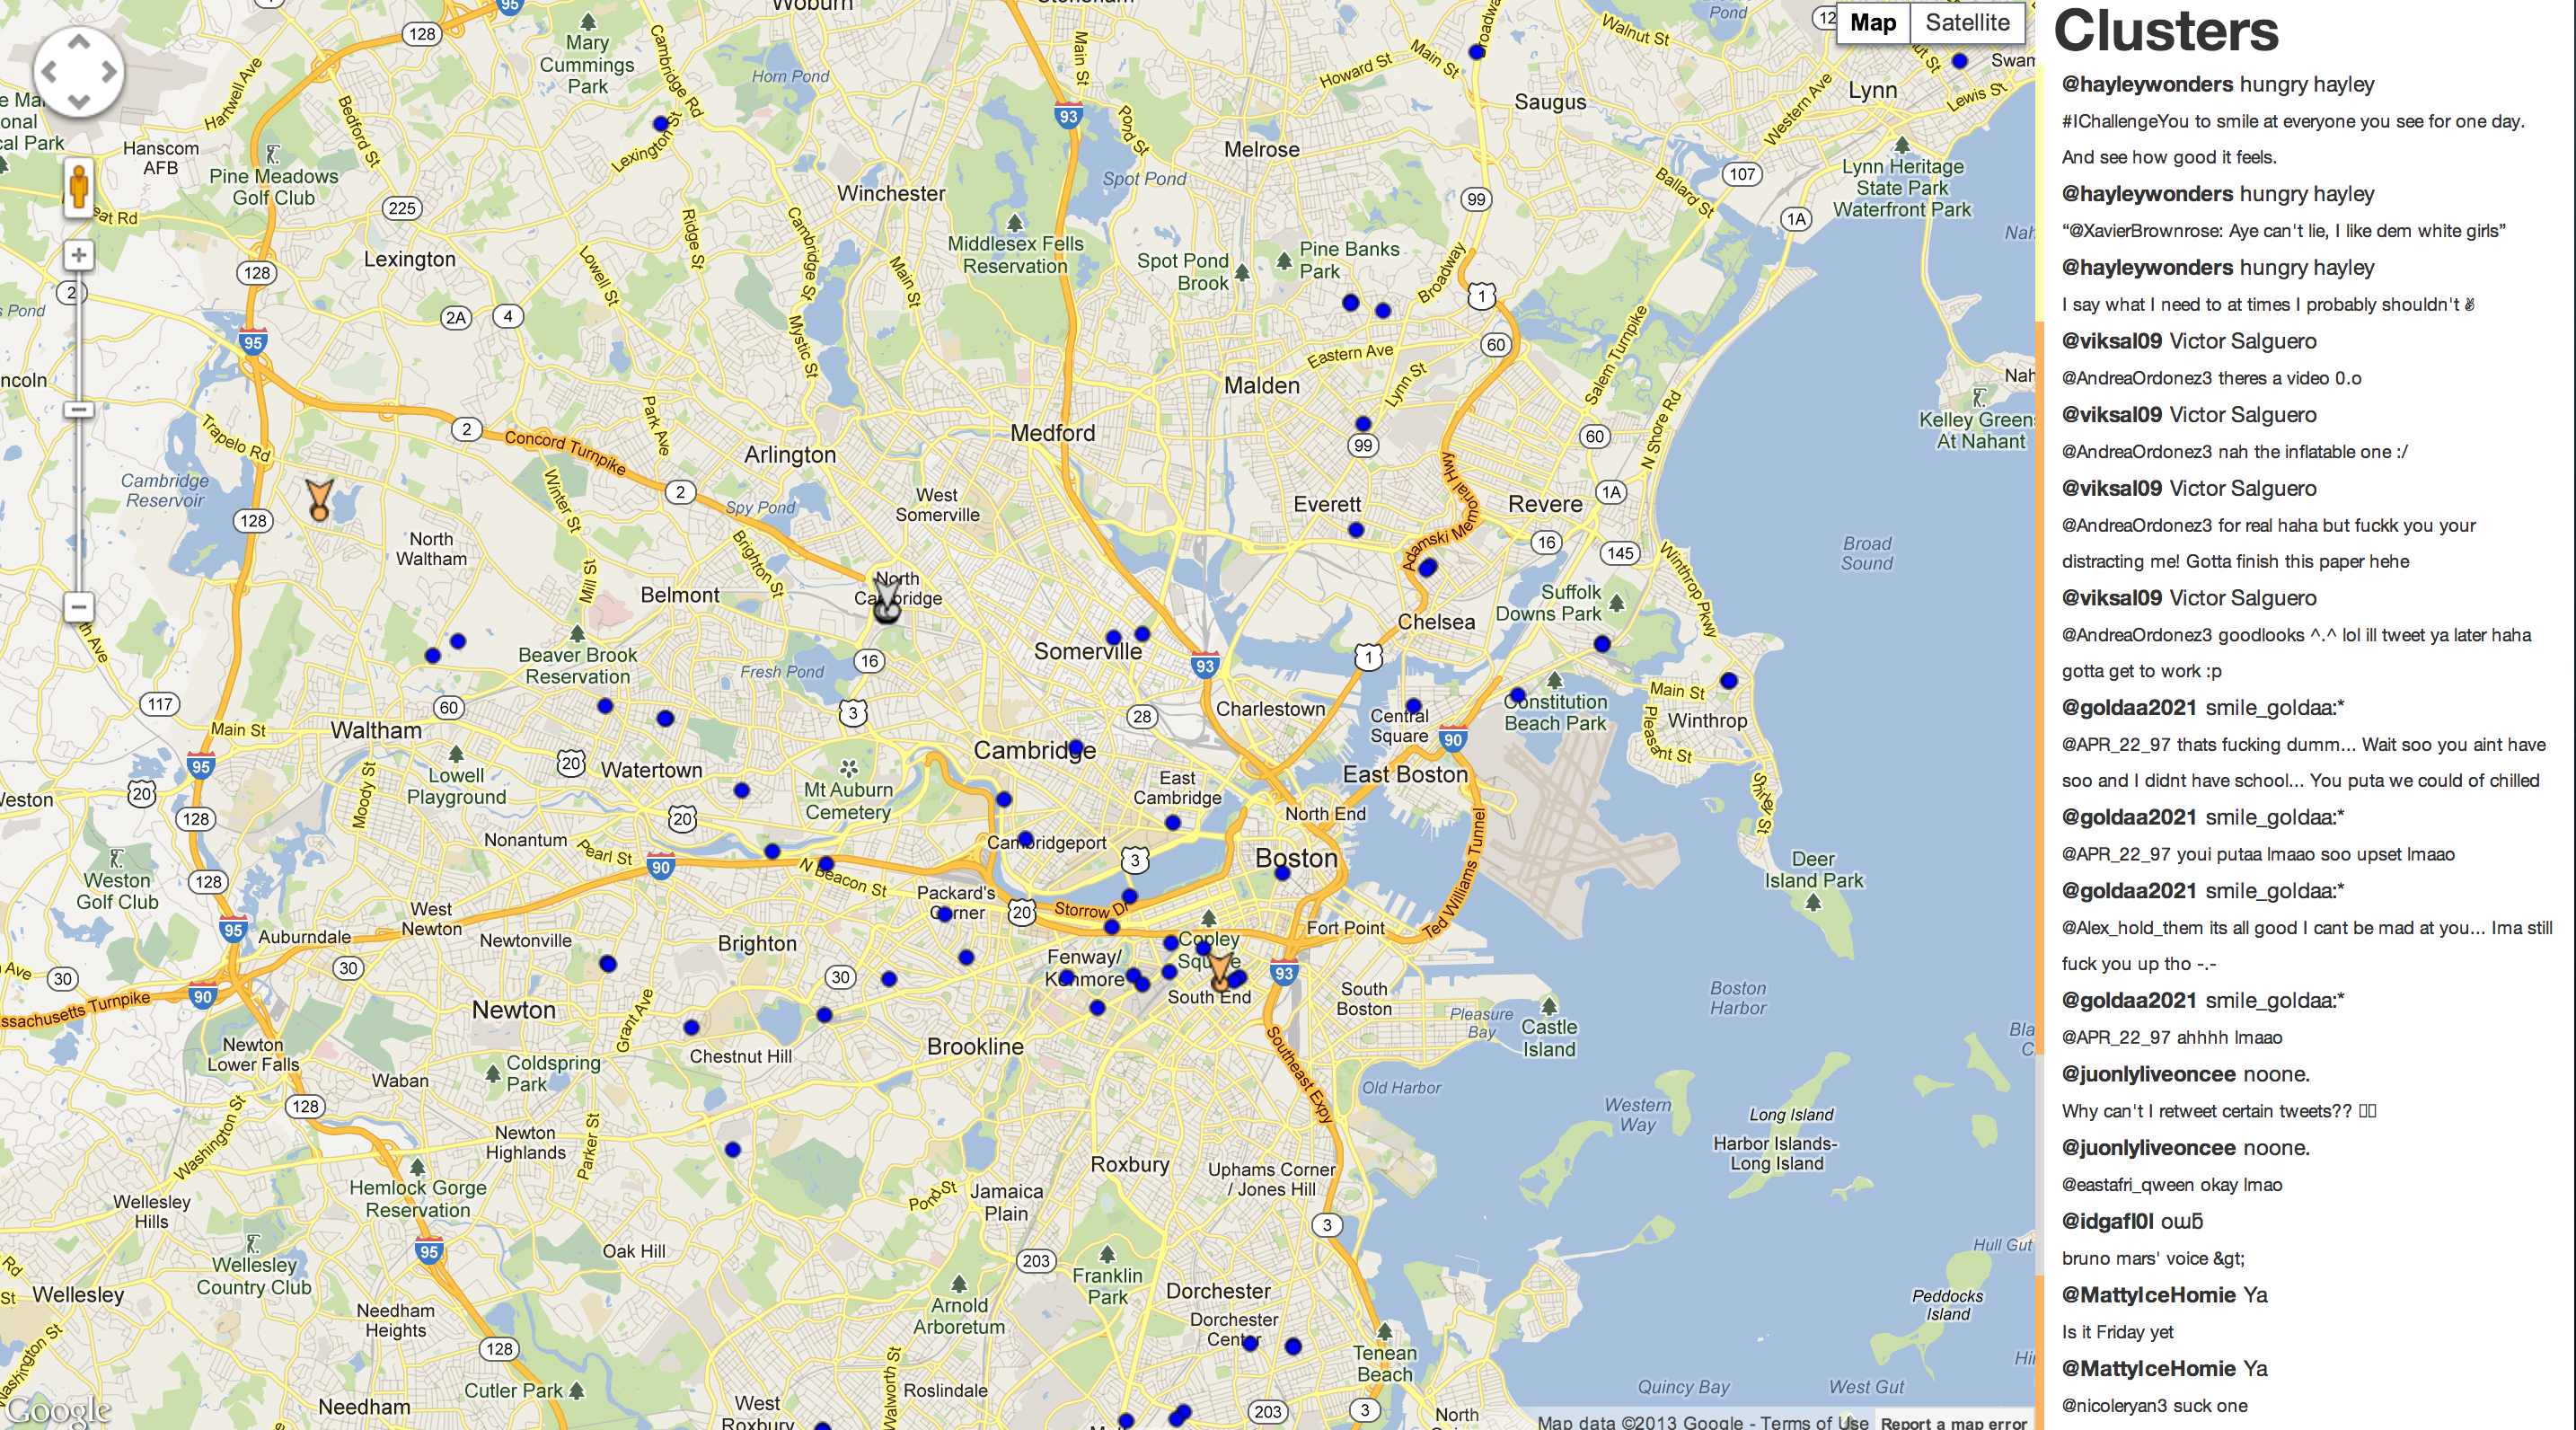
\includegraphics[width=5.5in]{hover2.png} \\ \\
Not only does this allow viewers to brush clusters effectively, it also further assists with the visual query of actually associating a cluster of tweets listed on the sidebar with a location on the map.

\section{Visualizations and Discussion} 
\subsection{Visualization}
Our visualization allows the user to select a geography of interest, and to draw tweets on the map in real time. By default, our visualization is currently focused on Boston; however, users can zoom and drag the map as desired to grab tweets from any particular region in the world. As data arrives, we also dynamically detect clusters of interesting points in the current viewport/geography, and visually group them by enclosing them in a circle and coloring them similarly. In addition, we display a list of all the identified clusters, and the component tweets in each cluster, in a secondary view - a sidebar to the the right of the map. Our visualization also supports several user interactions, as described below:
\begin{enumerate}
\item Linking \& Brushing. Our visualization has two views, the map - which displays the geographical location of tweets and clusters - and the cluster sidebar - which contains a list of all clusters currently identified and the member tweets of each cluster. We support linking \& brushing by interactively highlighting the cluster marker on the map (by making it larger) when ther viewer hovers over the cluster in the cluster sidebar. 
\item Details-on-Demand. Our visualization supports details-on-demand with a tool tip. Whenever a user hovers over an individual tweet on the map, regardless of whether or not it is in a cluster, a tool tip will appear after a short delay showing the text contained in the tweet. 
\item Drill-Down/Filter Capability. Our visualization suuports a drill-down or filtering interaction by allowing users to drag the map viewport and zoom in or out of the viewport as desired. In this way, the user can exactly specify what geographical area they wish to pull tweets and identify clusters in; the visualization responds by drilling-down/filtering tweets to match this specification.
\end{enumerate}

\subsection{Discussion}
The primary goal of our visualization was to identify events in the world as they were happening. At first, because our live twitter data stream only subsampled the true twitter ``firehose", we were concerned that we were not going to be able to find any clusters at certain zooms. Fortunately, in practice, our visualization identified several clusters with only a few minutes of streaming at a wide variety of zooms, from continent-level zoom (all of Africa), to country-level zoom (all of the US), to city-level zoom (Boston), and others. 

However, it is not immediately clear that the clusters we found correspond to real-world events. For example, some of the events that we found look something like this: \\ \\
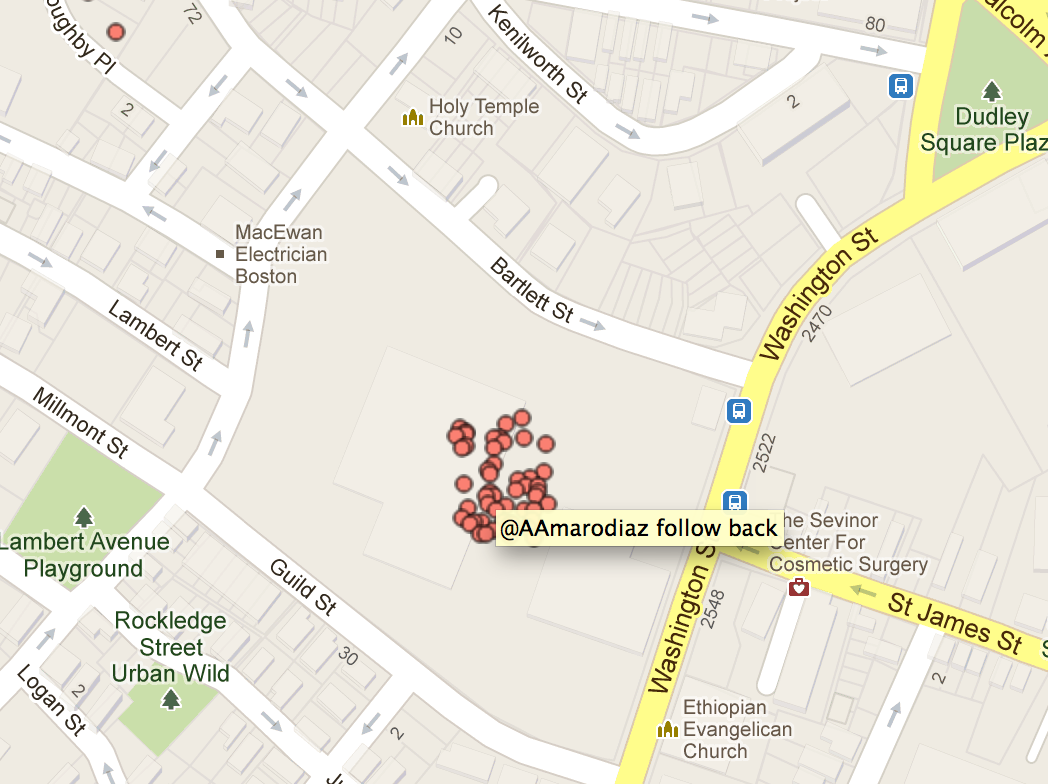
\includegraphics[width=5.5in]{lonely.png} \\ \\
This cluster is just one lonely soul, tweeting from the same location, trying to convince other people to follow him on twitter. We certainly wouldn't classify this as an event. However, a significant number of our clusters did end up corresponding to real-world events; we found a baseball game at Fenway: \\ \\
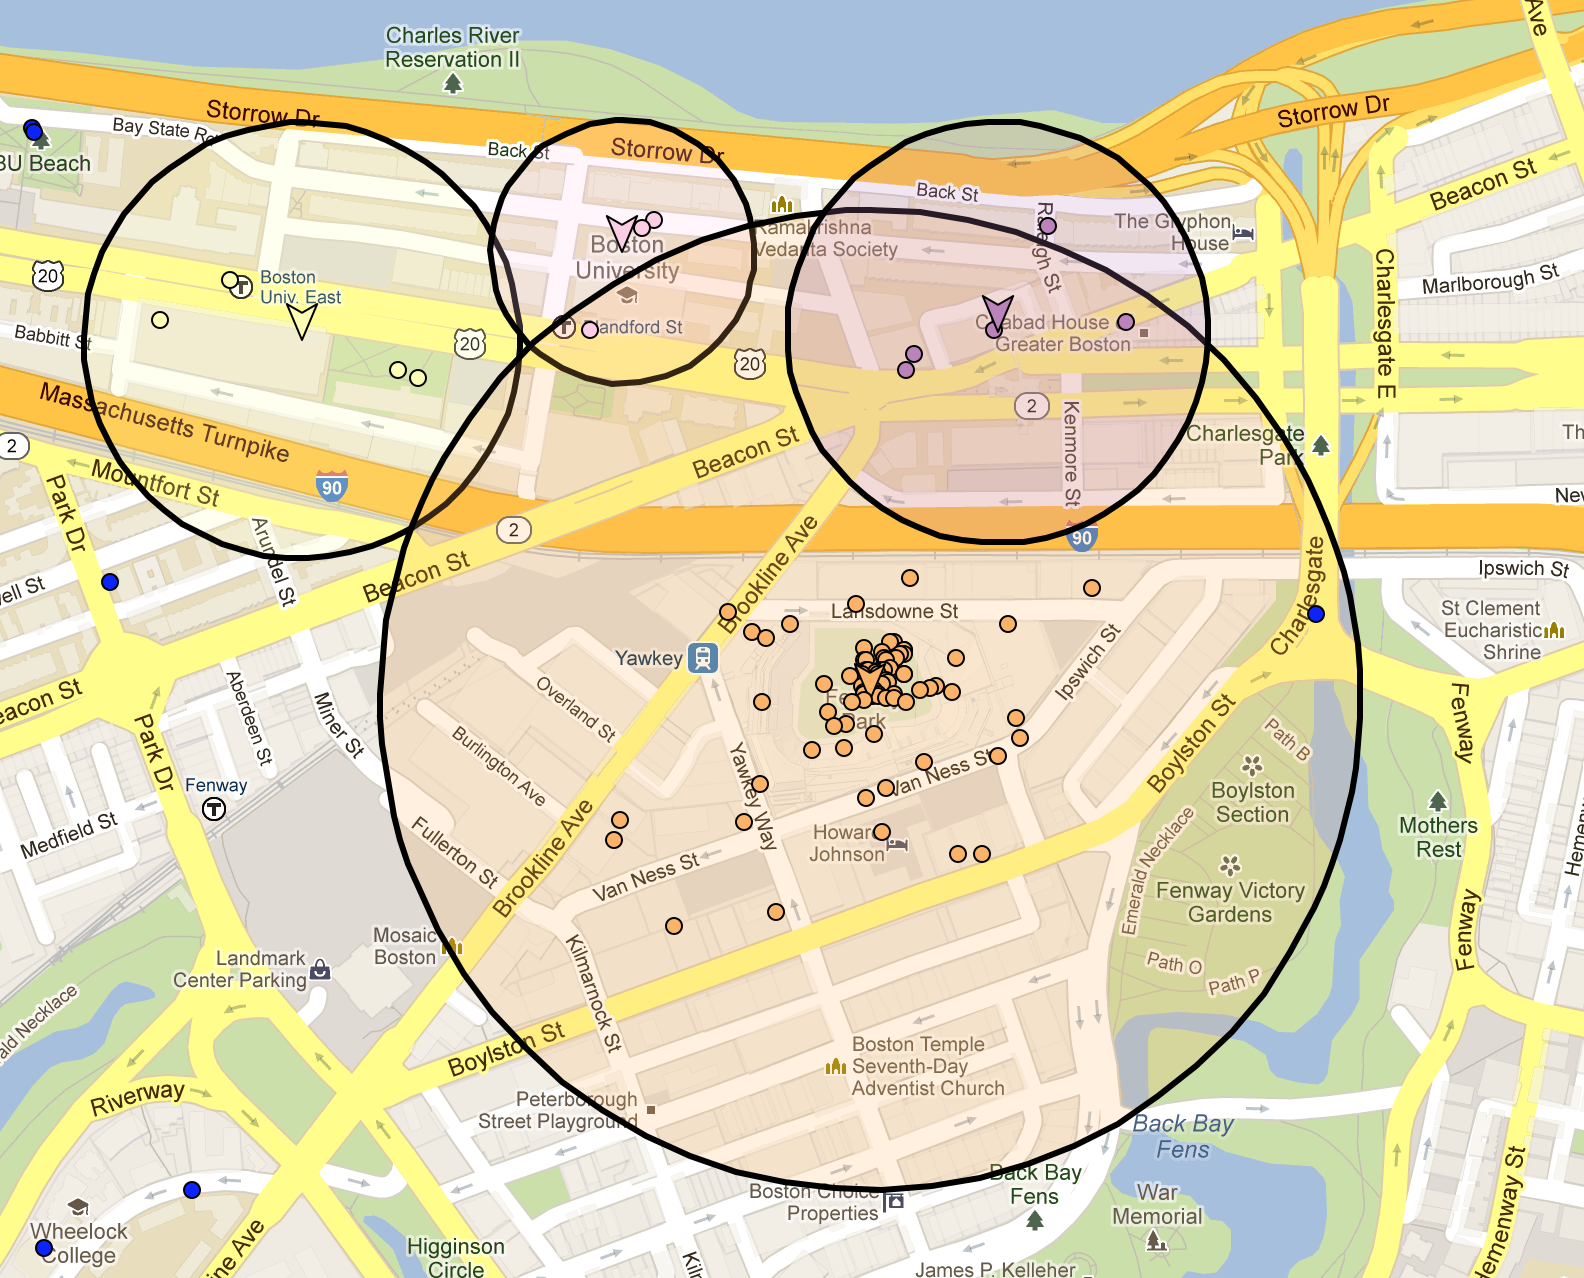
\includegraphics[width=5.5in]{fenway1.png} \\ \\
The fact that some of our clusters are not real events suggests that we can further improve our current visualization technique (discussed in the conclusion below). However, we did ultimately succeed in independently discovering events in the world that we were not aware of. We take this as a proof of concept; it is definitely possible to take a high-throughput social data streaming source, and identify events that are occurring in the real world. 

\section{Conclusion}
In Project 2, we implemented Pheme, a real-time social data visualization. Pheme demostrates that it is possible to identify real events by examining the instantaneous social data generated by people participating in the events. Furthermore, Pheme allows users to experience and visualize events all over the world, through the social data these events generate, on their home computer, in real time.

\subsection{Future Work}
In Project 3, we hope to improve on Pheme in several ways:
\begin{enumerate}
\item Refine our clustering algorithm to ignore certain types of non-events, including one individual tweeting rapidly. 
\item Extend our clustering algorithm to identify events using other closeness metrics, rather than just geographical closeness. We might consider tweets that we identify to be related through natural language processing, some metric related to time, etc.
\item Aggregate information about identified events, such as trying to determine what the event is about by analysing the constituent tweets, and pulling in data from that locale using other social data sources, like Instagram.
\item Implement reclustering. By doing so, we could allow users to drill down into one coarse event that they had discovered, and possibly find subevents within that event. For example, at a heavy-metal concert, one might discover a subevent in the mosh pit, and another behind the stage. 
\end{enumerate} 
\end{document}
